
\documentclass[12pt,letterpaper]{article}
\usepackage[utf8]{inputenc}
\usepackage{amsmath,amssymb}
\usepackage{float}
\usepackage{graphicx}
\usepackage[margin=2.54cm]{geometry}
\usepackage{enumerate}
\usepackage{xcolor}
\usepackage{physics}
\usepackage{caption}
\usepackage{fancyhdr}
\usepackage{pgfplots}
\usepackage{enumitem}
\usepackage{tikz}
\usepackage{tikz-3dplot} % Permite coordenadas 3D
\pagestyle{empty}
% Definir un comando para el número de pregunta en azul
\newcommand{\question}[1]{\textcolor{blue}{\textbf{#1}}}
%\newcommand{\abs}[1]{\lvert#1\rvert}
%\usepackage[spanish]{babel}
\setlength{\headheight}{14.5pt} % Ajustar la altura del encabezado
\usetikzlibrary{3d}
\pagestyle{fancy}
\fancyhf{}
\fancyhead[L]{Taller No. 4-Teoría Electromagnética}
\renewcommand{\footrulewidth}{0.4pt}
\pgfplotsset{compat=1.18}



\begin{document}
\begin{titlepage}
        \begin{center}
            \LARGE \textbf{Taller No. 3\\Teoría Electromagnética}
            \vfill
            \large

            Karen Alejandra Freire Rosero\\
            Sonier Andrés Ortiz Castelblanco\\
            Sarah Isabel Tejada García\\
            Santiago Alejandro Pérez Ramos
            \vfill
            \textbf{Asignatura:} Teoría Electromagnética\\
            \textbf{Profesor:} Servio Tulio Pérez Merchancano, Ph.D\\
            \vfill
            Universidad del Cauca\\
            Facultad de Ciencias Naturales, Exactas y de la Educación\\
            Departamento de Física\\
            Popayán, Cauca\\
            2025
        \end{center}
\end{titlepage}


 \section*{Problema 2.25:} Usando las Ecs. 2.27 y 2.30, encuentra el potencial a una distancia $z$ sobre el centro de las distribuciones de carga en la Fig. 2.34. En cada caso, calcula el campo eléctrico $\mathbf{E} = -\nabla V$, y compara tus respuestas con los Ej. 2.1, 2.2 y el Prob. 2.6, respectivamente. 

Supón que cambiamos la carga de la derecha en la Fig. 2.34a a $-q$; ¿cuál sería entonces el potencial en $P$? ¿Qué campo sugiere eso? Compara tu respuesta con el Prob. 2.2, y explica cuidadosamente cualquier discrepancia.


\begin{figure}[h] 
    \centering
    \includegraphics[width=0.7\textwidth]{imagenes/problema_25.png}
    \captionsetup{labelformat=empty}
    \label{Esquema}
\end{figure}

\subsection*{Solución}
\begin{itemize}
    \item Potencial debido a cargas puntuales (Ec. 2.27):
    \[
        V(\mathbf{r}) = \frac{1}{4\pi\varepsilon_0} \sum_i \frac{q_i}{|\mathbf{r} - \mathbf{r}_i|}
    \]
    \item Potencial debido a una distribución continua (Ec. 2.30):
    \[
        V(\mathbf{r}) = \frac{1}{4\pi\varepsilon_0} \int \frac{\rho(\mathbf{r'})}{|\mathbf{r} - \mathbf{r'}|} \, d\tau'
    \]
\end{itemize}

\subsection*{(a): Dos Cargas Puntuales}

Ubicación de las cargas:
\[
\mathbf{r}_1 = \left(-\frac{d}{2}, 0, 0\right), \quad \mathbf{r}_2 = \left(+\frac{d}{2}, 0, 0\right)
\]
Punto de observación:
\[
\mathbf{r} = (0, 0, z)
\]

Se tiene:
\[
\abs{\mathbf{r} - \mathbf{r}_1} = \sqrt{\left(\frac{d}{2}\right)^2 + z^2}, \quad \abs{\mathbf{r} - \mathbf{r}_2} = \sqrt{\left(\frac{d}{2}\right)^2 + z^2}
\]

\textbf{Potencial:}
\[
V = \frac{q}{4\pi\varepsilon_0} \left( \frac{1}{\abs{\mathbf{r} - \mathbf{r}_1}} + \frac{1}{\abs{\mathbf{r} - \mathbf{r}_2}} \right) \]

\[V= \frac{q}{2\pi\varepsilon_0 \sqrt{(d/2)^2 + z^2}}
\]

\textbf{Campo:}
Se tiene:
\[
\mathbf{E} = -\nabla V
\]

Dado que el punto está sobre el eje \(z\), solo se realiza  la derivada respecto a \(z\):
\[
E = -\pdv{V}{z} \hat{z}
\]
Entonces:
\[
E_z = -\frac{dV}{dz} 
\]
\[
\mathbf{E}  -\frac{q}{2\pi \varepsilon_0} \, \frac{dV}{dz}  \left( \frac{1}{\sqrt{z^2 + \left( \frac{d}{2} \right)^2}} \right) \, \hat{z} \\
\]
\[
\mathbf{E} = -\frac{q}{2\pi \varepsilon_0} \left( -\frac{1}{2} \cdot \frac{2z}{\left[ z^2 + \left( \frac{d}{2} \right)^2 \right]^{3/2}} \right) \, \hat{z} \\
\]
\[
\mathbf{E}= \frac{qz}{2\pi \varepsilon_0 \left[ z^2 + \left( \frac{d}{2} \right)^2 \right]^{3/2}} \, \hat{z} 
\]
Se puede ver que el resultado concuerda con el ejemplo 2.1

\subsection*{Caso adicional: una carga es $-q$}


Supongamos ahora que la carga del lado derecho en el inciso (a) es \(-q\). Entonces, el potencial en el eje \(z\) es:

\[
V = \frac{1}{4\pi\varepsilon_0} \left( \frac{q}{\sqrt{z^2 + (d/2)^2}} - \frac{q}{\sqrt{z^2 + (d/2)^2}} \right) = 0
\]

Donde:

\[
\mathbf{E} = -\nabla V = 0
\]

Pero esto entra en contradicción con la respuesta del Problema 2.2.Para este caso solo se conoce  \(V\) en el eje \(z\), y con eso no se puede calcular \(E_x = -\partial V/\partial x\) ni \(E_y = -\partial V/\partial y\).

Esto era aceptable en el caso original (a) porque, por simetría, sabíamos que \(E_x = E_y = 0\), y por lo tanto todo el campo apuntaba en la dirección \(\hat{z}\). Sin embargo, al cambiar una de las cargas a \(-q\), el sistema ya no es simétrico respecto al eje \(z\), y ahora el campo eléctrico apunta en la dirección \(x\).

\subsection*{(b) Línea de carga uniforme}

Elemento de carga:
\[
dq = \lambda \, dx
\]

Vector fuente:
\[
\mathbf{r}' = (x, 0, 0), \quad \mathbf{r} = (0, 0, z)
\]

\[
\abs{\mathbf{r} - \mathbf{r}'} = \sqrt{x^2 + z^2}
\]

\textbf{Potencial:}
\[
V(z) = \frac{1}{4\pi\varepsilon_0} \int_{-L}^{L} \frac{\lambda \, dx}{\sqrt{x^2 + z^2}} 
\]
\[
\int \frac{dx}{\sqrt{x^2 + z^2}} = \ln\left(x + \sqrt{x^2 + z^2} \right)
\]

Aplicando los límites:

\[
V(z) = \frac{\lambda}{4\pi \varepsilon_0} \left[ \ln\left(x + \sqrt{x^2 + z^2}\right) \right]_{-L}^{L}
\]

\[
V(z) = \frac{\lambda}{4\pi \varepsilon_0} \left[ \ln\left(L + \sqrt{L^2 + z^2} \right) - \ln\left(-L + \sqrt{L^2 + z^2} \right) \right]
\]

Usando propiedades logarítmicas:

\[
V(z) = \frac{\lambda}{4\pi \varepsilon_0} \ln\left( \frac{L + \sqrt{L^2 + z^2}}{-L + \sqrt{L^2 + z^2}} \right)
\]

Multiplicando numerador y denominador por el conjugado:

\[
V(z) = \frac{\lambda}{2\pi \varepsilon_0} \ln\left( \frac{L + \sqrt{L^2 + z^2}}{z} \right)
\]

\textbf{Campo Eléctrico:}

\[
E_z = -\frac{dV}{dz}
\]


Usamos la regla de derivación de un logaritmo de cociente:

\[
\frac{d}{dz} \ln\left( \frac{f(z)}{g(z)} \right) = \frac{f'(z)}{f(z)} - \frac{g'(z)}{g(z)}
\]

Donde:

\(f(z) = L + \sqrt{L^2 + z^2} \Rightarrow f'(z) = \frac{z}{\sqrt{L^2 + z^2}}\)

\(g(z) = z \Rightarrow g'(z) = 1\)

Entonces:

\[
\frac{dV}{dz} = \frac{\lambda}{2\pi \varepsilon_0} \left( \frac{z}{(L + \sqrt{L^2 + z^2}) \sqrt{L^2 + z^2}} - \frac{1}{z} \right)
\]

Por tanto, el campo eléctrico en la dirección \(\hat{z}\) es:

\[
\mathbf{E} = - \frac{\lambda}{2\pi \varepsilon_0} \left( \frac{z}{(L + \sqrt{L^2 + z^2}) \sqrt{L^2 + z^2}} - \frac{1}{z} \right) \hat{z}
\]

Se puede ver que el resultado concuerda con el ejemplo 2.2

\subsection*{(c): Disco con Carga Superficial Uniforme}


Elemento de carga:
\[
dA = r\,dr\,d\phi
\]
\[
dq = \sigma \, dA = \sigma  r\,dr\,d\phi
\]

Punto de observación: \(\mathbf{r} = (0, 0, z)\)

Vector fuente: \(\mathbf{r}' = (r \cos\theta, r \sin\theta, 0)\)

\[
{\mathbf{r} - \mathbf{r}'} = \sqrt{r^2 + z^2}
\]

\textbf{Potencial:}

\[
V = \frac{1}{4\pi\varepsilon_0} \int_0^{2\pi} \int_0^R \frac{\sigma\, r\, dr\, d\phi}{\sqrt{z^2 + r^2}}
\]

\[
V = \frac{\sigma}{4\pi\varepsilon_0} \int_0^R \int_0^{2\pi} \frac{r\, d\phi\, dr}{\sqrt{z^2 + r^2}}
\]

\[
V = \frac{\sigma}{4\pi\varepsilon_0} \int_0^R \frac{2\pi r\, dr}{\sqrt{z^2 + r^2}}
= \frac{2\pi\sigma}{4\pi\varepsilon_0} \int_0^R \frac{r\, dr}{\sqrt{z^2 + r^2}}
\]
Sustituyendo:

\[
u = z^2 + r^2 \Rightarrow du = 2r\, dr \Rightarrow r\, dr = \frac{du}{2}
\]

\[
V = \frac{2\pi\sigma}{4\pi\varepsilon_0} \int_0^R u^{-1/2} \frac{du}{2r}
\]

\[
V = \frac{\pi \sigma}{4\pi \varepsilon_0} \int_0^R u^{-1/2} \, du
\]

\[
V = \frac{\sigma}{4\varepsilon_0} \left[ 2u^{1/2} \right]_0^{R}
\]

\[
V = \frac{\sigma}{2\varepsilon_0} \left[ \sqrt{z^2 + R^2} - z \right]
\]
\textbf{Campo:}
\[
E_z = -\frac{dV}{dz}
\]
\[
E = -\frac{d}{dz} \left[ \frac{\sigma}{2\varepsilon_0} \left( \sqrt{z^2 + R^2} - z \right) \right]
\]

\[
E = -\frac{\sigma}{2\varepsilon_0} \left( \frac{d}{dz} \sqrt{z^2 + R^2} - \frac{d}{dz} z \right)
\]

\[
E = -\frac{\sigma}{2\varepsilon_0} \left( \frac{z}{\sqrt{z^2 + R^2}} - 1 \right)
\]

\[
\mathbf{E} = \frac{\sigma}{2\varepsilon_0} \left( 1 - \frac{z}{\sqrt{z^2 + R^2}} \right) \hat{z}
\]
Se puede ver que el resultado concuerda con el problema 2.6

%------------------------------------------------------------------------------------


\section*{\question{Problema 26 } }
Una superficie cónica (como un cono de helado vacío) tiene una densidad superficial de carga uniforme 
$\sigma$. La altura del cono es h, al igual que el radio de la parte superior. Encuentra la diferencia de potencial entre los puntos a (el vértice del cono) y b (el centro de la parte superior).

\begin{figure}[ht]
  \begin{center}
  
    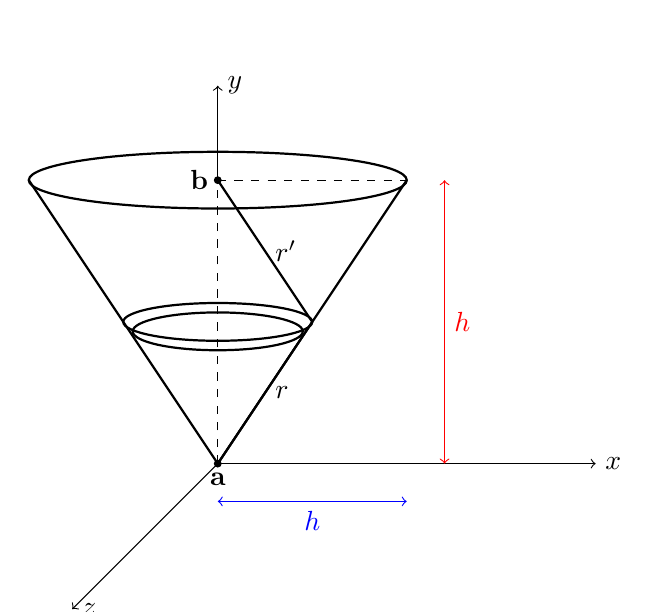
\begin{tikzpicture}[scale=1.2]
        % Eje vertical
        \draw[->] (0,0,0) -- (0,0,4) node[anchor=west] {$z$};
        \draw[->] (0,3,0) -- (0,4,0) node[anchor=west] {$y$};
        \draw[->] (0,0,0) -- (4,0,0) node[anchor=west] {$x$};

        % Cono
        \draw[thick] (0,0) -- (-2,3);
        \draw[thick] (0,0) -- (2,3);
        \draw[thick] (0,3) ellipse (2 and 0.3); % Borde superior del cono
        \draw[thick] (0,1.5) ellipse (1 and 0.2); %elemento diferencial de área 
        \draw[thick] (0,1.4) ellipse (0.9 and 0.2); % elemento diferencial de área
        \draw[thick] (1,1.5) -- (0,3) node[midway,right] {$r'$};
        \draw[thick] (0,0) -- (1,1.5) node[midway,right] {$r$};
        \filldraw[black] (0,0) circle (1pt) node[anchor=north] {$\mathbf{a}$ };
        \filldraw[black] (0,3) circle (1pt) node[anchor=east] {$\mathbf{b}$ };

        % Altura h
        \draw[<->,red] (2.4,0) -- (2.4,3) node[midway, right] {$h$};

        % Radio h
        \draw[<->,blue] (0,-0.4) -- (2,-0.4) node[midway, below] {$h$};
        % segmentos 
        \draw[dashed] (0,3) -- (2,3); 
        \draw[dashed] (0,0) -- (0,3);

    \end{tikzpicture}
  \caption*{Superficie cónica }\label{fig:}
  \end{center}
\end{figure}
 
\subsection*{Solución}

El potencial eléctrico debido a una distribución superficial de carga es:
\[
  V(P)=\frac{1}{4\pi\varepsilon_0}\iint_{\mathcal{S}}\frac{\sigma\,da}{r},
\]
donde $r$ es la distancia desde el elemento de área $da$ hasta el punto $P$.

Sea $R$ la longitud de la generatriz del cono:
\[
  R=\sqrt{h^2+r^2}=\sqrt{h^2+h^2}=h\sqrt{2}.
\]
El elemoto diferencial de area $da$ en coordenadas esféricas es:

\[
  da = (r\sin\theta)\,drd\phi\, = \frac{r}{\sqrt{2}}\,drd\phi
\]
\subsection*{Potencial en el vértice $a$}
En el vértice $a$, la distancia desde un elemento $da$ hasta $a$ es $r$.

\begin{align*}
  V(a) &=\frac{1}{4\pi\varepsilon_0}\int_{0}^{2\pi}d\phi\int_{0}^{R}\frac{\sigma\,(r\sin\theta)\,dr}{r}\\
     &=\frac{2\pi\sigma}{4\pi\varepsilon_0} \frac{1}{\sqrt2}\int_{0}^{R}dr\\
     &=\frac{\sigma}{2\varepsilon_0}\frac{1}{\sqrt2}R\, \,\, ,Donde \, R=\sqrt2h\\
     &=\frac{\sigma}{2\varepsilon_0}\frac{1}{\sqrt2}\,h\sqrt2\\
     &=\frac{\sigma\,h}{2\varepsilon_0}.
\end{align*}

\section*{Potencial en el centro de la base $b$}
En el centro de la base $b$, situado sobre el eje del cono a una distancia $h$ del vértice, la distancia a un punto de la superficie es:

\begin{figure}[h!]
  \centering
  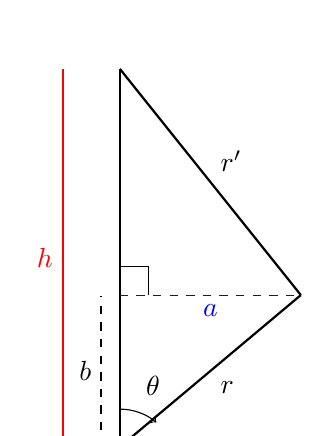
\begin{tikzpicture}[scale=1.2]
    % Parámetros numéricos para el dibujo
    \def\r{2.5}      % valor arbitrario de r
    \def\h{4}        % valor arbitrario de h
    \def\ang{50}   % ángulo θ en grados
    \pgfmathsetmacro{\b}{\r*cos(\ang}  % b = r cosθ
    \pgfmathsetmacro{\a}{\r*sin(\ang}  % a = r sinθ

    % Puntos clave
    \coordinate (A) at (0,0);
    \coordinate (D) at (0,\b);
    \coordinate (B) at (0,\h);
    \coordinate (C) at (\a,\b);

    % Lados del triángulo ABC
    \draw[thick] (0,0) -- (0,4);
    \draw[thick,red] (-0.6,0) -- (-0.6,4) node[midway,left] {$h$};
    \draw[thick] (B) -- (C) node[midway,above right] {$r'$};
    \draw[thick] (A) -- (C) node[midway,below right] {$r$};

    % Proyecciones a y b (líneas punteadas)
    \draw[dashed,blue] (D) -- (C) node[midway,below] {$a$};
    \draw[dashed] (-0.2,0) -- (-0.2,1.6) node[midway,left] {$b$};

    % Indicación de ángulo recto en D
    \draw ($(D)+(0,0.3)$) -- ++(0.3,0) -- ++(0,-0.3);

    % Ángulo θ en A
    \draw[->] (A) ++(0,0.4) arc[start angle=90,end angle=\ang,radius=0.6];
    \node at ($(A)+(0.35,0.65)$) {$\theta$};

    % Etiqueta de r sinθ y r cosθ (opcional)
    %\node at ($(D)+(0.5,\b*0.3)$) {$r\sin\theta$};
    %\node at ($(A)+( -0.6,\b/2)$) {$r\cos\theta$};
  \end{tikzpicture}
  \caption*{Triángulo con lados \(r\), \(h\) y \(r'\), y sus proyecciones \(a\) y \(b\).}
  \label{fig:leycos}
\end{figure}

En el triángulo superior de la se tiene un ángulo recto en, luego por pitàgoras 
\[
  r'^2 \;=\; a^2 + (h - b)^2.
\]
Definición de proyecciones en el triángulo
\[
  a \;=\; r\sin\theta
  \quad\text{y}\quad
  b \;=\; r\cos\theta.
\]
Sustituyendo,
\begin{align*}
  r'^2 & =\, (r\sin\theta)^2 + \bigl(h - r\cos\theta\bigr)^2\\
     &=\, r^2\sin^2\theta + h^2 + r^2\cos^2\theta - 2hr\cos\theta\\
     &=\, r^2 + h^2 - 2\,h\,r\cos\theta,
\end{align*}
  
Por lo tanto la distancia \(r'\) entre el punto \(b\) y un elemento de carga \(da\) en la superficie del cono es:
\(\;r'^2 = r^2 + h^2 - 2rh\cos\theta.\)
\[
  r'=\sqrt{r^2 + h^2 - 2hr\cos\theta} , \,\,\,\,\,\theta = \pi/4
\]
\[
r'(r)=\sqrt{r^2 + h^2 - \sqrt2\,h\,r }.
\]
Por tanto:
\begin{align*}
V(b)
&=\frac{1}{4\pi\varepsilon_0}\int_{0}^{R}\frac{\sigma\,(2\pi\,r\sin\theta)\,dr}{r'(r)}\\
&=\frac{\sigma\sin\theta}{2\varepsilon_0}\int_{0}^{R}\frac{r\,dr}{\sqrt{r^2 - \sqrt2\,h\,r + h^2}}.
\end{align*}
Para evaluar la integral, completamos el cuadrado:
\[
  r^2 - \sqrt2\,h\,r + h^2
  =\Bigl(r-\tfrac{h}{\sqrt2}\Bigr)^2 + \tfrac{h^2}{2}.
\]
Con el cambio $u=r-\tfrac{h}{\sqrt2}$, $dr=du$, $u\in[-h/\sqrt2,\,h/\sqrt2]$,
\[
\int_{0}^{R}\frac{r\,dr}{\sqrt{(r-\tfrac{h}{\sqrt2})^2+\tfrac{h^2}{2}}}
=\int_{-h/\sqrt2}^{h/\sqrt2}\frac{u+\tfrac{h}{\sqrt2}}{\sqrt{u^2+\tfrac{h^2}{2}}}\,du
=I_1+I_2,
\]
Resolviendo la integral \(I_1\):
\begin{align*}
  I_1&=\int_{-h/\sqrt2}^{h/\sqrt2}\frac{u\,du}{\sqrt{u^2+\tfrac{h^2}{2}}}\\ 
     & =\Bigl[ \sqrt{u^2+h^2/2}\Bigr]_{-h/\sqrt2}^{h/\sqrt2}\\
     & =h-h\\
     & = 0
\end{align*}
Resolviendo la integral \(I_2\):
\[
I_2 = \frac{h}{\sqrt2}
\int_{-\,\frac{h}{\sqrt2}}^{+\,\frac{h}{\sqrt2}}
\frac{du}{\sqrt{u^2 + \bigl(\tfrac{h}{\sqrt2}\bigr)^2}}
\]
Sea 
\[
u = \frac{h}{\sqrt2}\,\tan\theta,d\,\,\,\,u = \frac{h}{\sqrt2}\,\sec^2\theta,d\,\,\,\theta\,\,\,\, \sqrt{u^2 + \bigl(\tfrac{h}{\sqrt2}\bigr)^2} = \frac{h}{\sqrt2}\,\sec\theta,\\[6pt]
\]
\[
\theta_1 = \arctan\!\bigl(-1\bigr) = -\tfrac\pi4,
\theta_2 = \arctan\!(+1) = +\tfrac\pi4,
\]

\begin{align*}
I_2
&= \frac{h}{\sqrt2}
    \int_{\theta_1}^{\theta_2}
      \frac{\frac{h}{\sqrt2}\,\sec^2\theta\,d\theta}
           {\frac{h}{\sqrt2}\,\sec\theta}
\\
&= \frac{h}{\sqrt2}
    \int_{-\pi/4}^{\pi/4}
      \sec\theta\,d\theta
\\
&= \frac{h}{\sqrt2}
    \Bigl[\ln\bigl|\sec\theta + \tan\theta\bigr|\Bigr]_{-\pi/4}^{\pi/4}
\\
&= \frac{h}{\sqrt2}\Bigl(
      \ln\bigl(\sqrt2+1\bigr)
    - \ln\bigl(\sqrt2-1\bigr)
    \Bigr)
\\
&= \frac{h}{\sqrt2}\ln\!\frac{\sqrt2+1}{\sqrt2-1}
\\
&= \frac{h}{\sqrt2}\ln\!\bigl((\sqrt2+1)^2\bigr)
\end{align*}
Se obtiene:
\[
I_2 = \frac{2h}{\sqrt2}\ln(\sqrt2+1).
\]
Por tanto
\[
V(b)
=\frac{\sigma\sin\theta}{2\varepsilon_0}I_2
=\frac{\sigma\,h}{2\varepsilon_0}\ln(\sqrt2+1).
\]

\section*{Diferencia de potencial}
Finalmente
\[
V(a)-V(b)
=\frac{\sigma\,h}{2\varepsilon_0}
-\frac{\sigma\,h}{2\varepsilon_0}\ln(\sqrt2+1)
\]
\[
\boxed{V(a)-V(b)=\frac{\sigma\,h}{2\varepsilon_0}\Bigl(1-\ln(\sqrt2+1)\Bigr).}
\]
\end{document}
